% Preamble
\documentclass[11pt]{article}

% Packages
\usepackage{amsmath}
\usepackage{graphicx}

% Document
\begin{document}
    \section{Structure from Motion Algorithm}
    Structure from Motion is the task of calculating the 3D structure of a scene and the pose of cameras from
    images captured in multiple views or video frames. In this thesis, Incremental Structure from Motion, \cite{7780814}, will be explained
    as it is the base algorithm for most papers in these criteria.

    \begin{figure}
    \centering
    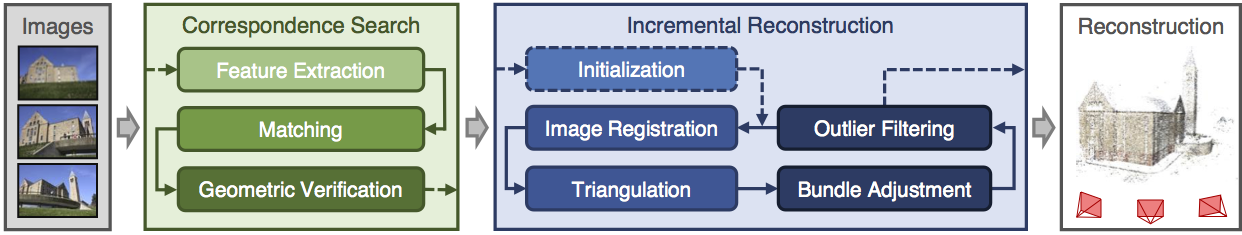
\includegraphics[width=\textwidth,height=\textheight,keepaspectratio]{images/sfm.png}
    \caption{An overview of Structure from Motion Revisited, \cite{7780814} pipeline}
    \end{figure}

    The algorithm can be viewed as a pipeline that contains the following separate steps:

    \begin{enumerate}
        \item \textbf{Feature detection and matching:} The first step in SFM is feature detection and matching, where
        the algorithm identifies common features or points in the 2D images or video frames. These features
        can be edges, corners, blobs, or other distinctive patterns that can be detected consistently across
        the images. The algorithm, then, matches these features between different input frames. This step is one
        of the most challenging parts in SfM. Occlusion, illumination changes, perspective transformation, and moving objects
        are some of them. However, since this is a core task in many Computer Vision tasks, there has been
        tons of research in feature detection and matching, including deep based approaches. SIFT (\cite{lowe1999object}), SuperPoint (\cite{detone2018superpoint}),
        D2-Net (\cite{dusmanu2019d2net}), R2D2 (\cite{revaud2019r2d2}) are often used among SfM related papers which
        will be described briefly in the next chapter.

        \item \textbf{Geometric Verification:} Raw matches are not enough for the scene reconstruction.
        Matches in similar repeated patterns, multiple the same objects in one image, etc, are some issues that may cause wrong
        poses and 3D points. So, outliers must be removed from the list of matches. By using the existing matches and
        epipolar geometry, camera matrices(i.e. H, F, and E matrices) are calculated.
        Then, the rest of the matches are verified by checking the geometric consistency of the reconstructed 3D points and
        camera poses. If they do not result in the same poses, they are filtered out. Having more matches is good.
        But, not all of them can be used.

        \item \textbf{Reconstruction Initialization:} If the pipeline is considered as an iterative or sequential process,
        a starting point is essential. Choosing a good initial pair of images is, so important. At the end of
        each iteration, the camera parameters and 3D structure are optimized. Without a good initial estimate,
        the optimization process usually doesn't converge and is stuck in local minima. A good initial pair usually is
        chosen from the images with the highest number of matches.

        \item \textbf{Image Registration and Triangulation:} After initialization, the algorithm calculates the
        camera pose for the new image by methods in section \ref{stereo_cameras} and uses triangulation to estimate
        the 3D position of the matched features in every new image. Triangulation is the process of finding the intersection point
        of two or more vectors that originate from the center of the camera and pass through the 2D features. The intersection
        point represents the 3D position of the feature in the scene.

        \item \textbf{Bundle Adjustment:} As the previous processes involve some errors. There are inconsistencies
        and misalignments between the estimated camera parameters and the triangulated 3D points, and since the algorithm
        is incremental, the errors are accumulated for every new image. Bundle adjustment refines those parameters by
        minimizing the non-linear reprojection equations. For each generated 3D point, its 3D coordinates are
        transformed into the corresponding 2D image coordinates using the estimated camera projection matrix.
        Then, the difference between the observed 2D projection and the reprojected 2D coordinates is considered as the error.
        Levenberg-Marquardt algorithm is usually used to minimize the error.
        The optimization problem can be high-dimensional, and it may take a long time to converge to a good solution.
        Nonetheless, bundle adjustment can significantly improve the accuracy of the reconstructed 3D scene and camera poses.

    \end{enumerate}

    \section{Related Works}
    Structure of Motion is a core task for many other projects. The accuracy and speed
    of the algorithm is crucial. For instance, even a minor rotation error of 1 degree in the camera can lead
    to significant misalignment of point coordinates in meters, particularly in open scenes. Also, during our
    experiment, it is observed that the pipeline fails in the initialization step for a considerable number of attempts
    because of the lack of correct matches.
    Therefore, over the past few decades, there have been lots of efforts to improve each part of these algorithms.
    Here is a review of the recent best papers in this area:

    \subsection{Researches in Feature Matching}
    The first step in SfM pipeline is feature matching which
    is one of the core tasks in many Computer Vision applications as they are used to identify the corresponding
    matches among the input images. Some of the challenges are deformation in different viewpoints, occlusion,
    illumination changes, moving objects, etc. There have been a lot of research in this area:

    \paragraph{Multi-View Optimization of Local Feature Geometry} (~\cite{Dusmanu2020Multi}) refines the existing keypoints. It tracks each keypoint in all input images and creates a tentative
    matches graph with keypoints as nodes and matches as edges. Each keypoint is known by its surrounding pixels
    information. So, a h*w patch is selected around the feature and a "d" dimensional descriptor is calculated by
    a neural network with Siamese architecture. Then, for each pixel, a dot product similarity is calculated
    with every pixel in the other patch (h*w*h*w dimension). After normalization, the pixel that has the most
    similarity value with keypoint is supposed to be selected, and the translation vector ($T_{u->v}$)
    moves the keypoint to the selected pixel. In the next stage, since each keypoint could be seen in multiple images,
    a single incorrect match or displacement can cause a cascade of errors in the results. Therefore, for each track of
    matches, a non-linear equation for minimizing the dot similarity between patches among all patches for the same
    keypoint is optimized. The idea of this paper is also used in \cite{lindenberger2021pixsfm} which will be
    described in detail in the next chapter.

    \begin{figure}
    \centering
    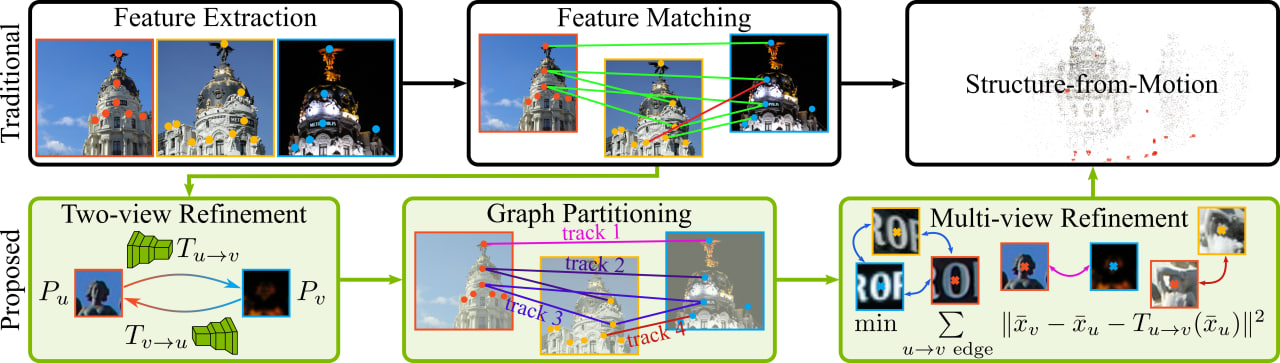
\includegraphics[width=\textwidth,height=\textheight,keepaspectratio]{images/dusmano.jpg}
    \caption{Paper: Multi-View Optimization of Local Feature Geometry, \cite{Dusmanu2020Multi}}
    \end{figure}

    \paragraph{Deep Two-View Structure-from-Motion Revisited} (~\cite{wang2021deep}) uses optical flow to predict
    dense matches between two frames. They use DICLFlow, explained in \cite{wang2020displacement} to generate
    dense matching points between two consecutive frames. Before calculating the essential matrix, noisy matches
    like moving objects are filtered out. They assumed that optical flow is more accurate in rich textured areas.
    So, they used SIFT method to detect less textured areas in order to mask out the optical flow there.
    Then, the essential matrix is calculated using the classic five-point algorithm with RANSAC, and
    the dense depth map is computed by performing triangulation. Before this process, the matching is performed
    for the second time by constraining the search space to epipolar lines computed from the relative camera poses.
    They filtered out noisy matches twice which means dense matches by optical flow are too noisy. Higher number of matches is good
    for obtaining more points in sparse reconstruction. However, they tend to be noisy. They also,
    introduced a Scale-Invariant Depth Module to deal with the up-to-scale relative pose and mismatch between the
    scale of the camera poses and the depth map. Up to scale problem means that while the
    relative positions of the reconstructed points are correct, their absolute positions in the real world
    are not known unless there is additional information, such as the size of an object in the scene or the
    distance between two known points. In order to deal with this problem, in each pair of images, this paper
    generates a number of matching candidates with different real world depths with the same interval per keypoint.
    And then, a plane-sweep powered network minimizes the loss function which is the position displacement of
    the features in the flow. This paper is able to find more and better matching points and therefore more
    accurate poses and depth maps, especially for textureless and occluded areas.

    \begin{figure}
    \centering
    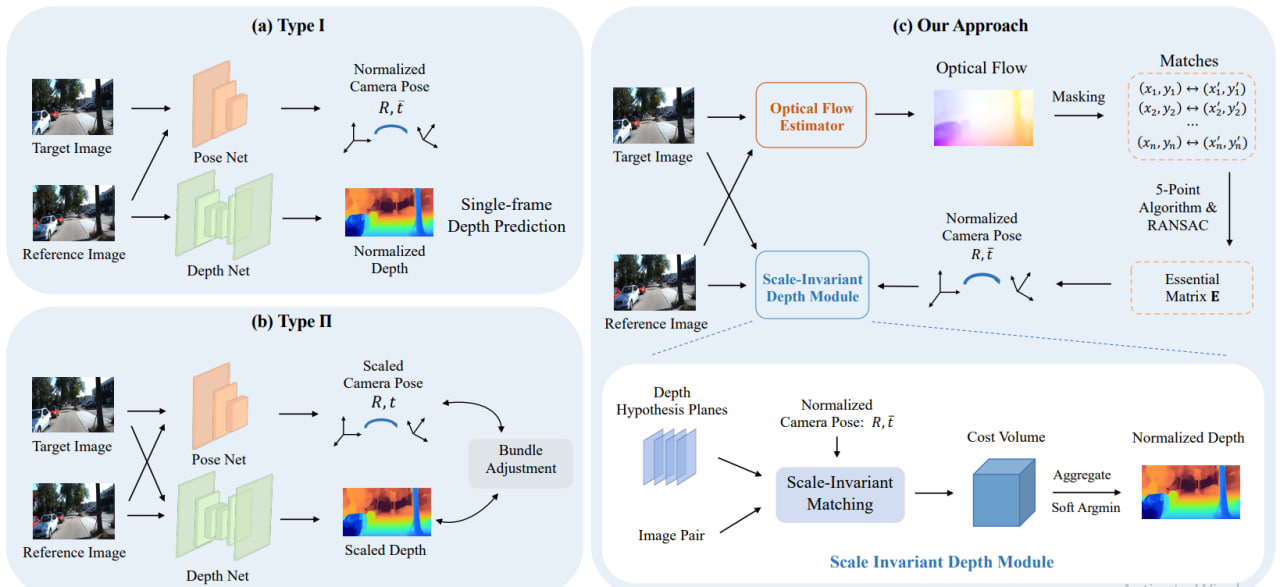
\includegraphics[width=\textwidth,height=\textheight,keepaspectratio]{images/deep_two_sfm.jpg}
    \caption{Paper: Deep Two-View Structure-from-Motion Revisited, \cite{wang2021deep}}
    \end{figure}

    \paragraph{} There is much more research in the feature matching step. \cite{revaud2019r2d2}, \cite{dusmanu2019d2net},
    and \cite{detone2018superpoint} are supervised deep learning based feature extractors that not only have
    outperformed handcrafted methods in terms of accuracy but also, could solve many challenges in this area like
    point of view challenges and multi-scale problems. Supervised learning means that the model has been trained
    based on the keypoints defined in the training dataset. Their problem is that they have less performance for features other
    than in the training dataset. Some of these papers have provided modules to train the model on your own customized features dataset

    \newpage
    \subsection{Researches in Bundle Adjustment}
    Bundle Adjustment algorithms optimize the camera parameters and the position of 3D points by minimizing the
    geometric errors between the projected 3D points and the corresponding 2D image observations, iteratively. However, there
    are some disadvantages to this technique. Bundle Adjustment requires solving a large system of
    non-linear equations, which can be computationally expensive, especially for large datasets. This can be a
    significant drawback, especially in real-time usage. In the experiment chapter, it will be shown that this is the most time-consuming part in Structure from Motion pipeline.
    Also, It is sensitive to the initial values. If the initial values are not accurate, the optimization may fail to converge.
    The optimization problem can have many local minima which means a high probability to converge to incorrect results.
    Also, the error may increase exponentially in the subsequent iterations. Here are some of the best papers focusing on these issues.

    \paragraph{BA-Net: Dense Bundle Adjustment Network} (~\cite{tang2019banet}) implemented feature-metric
    bundle adjustment that minimizes feature-metric errors instead of geometric erros between feature pyramids
    of images obtained by CNNs. As \cite{LSDSLAM} says, there are two types of BAs:
    \begin{enumerate}
        \item Typical geometric BA with re-projection error(pixel coordinates): Only a few pixels, i.e. keypoints, are taken into account which comes with keypoints detection and matching challenges
        \item Photometric BA algorithm(all aligned pixel, pixel intensities as error): It has good accuracy, especially at less textured scenes. However, the disadvantages would be sensitivity to camera exposure, illumination changes, and outliers such as moving objects. Also, considering all pixels would increase the computation dramatically.
    \end{enumerate}
    BA-Net creates a pyramid of features for each image and aligns them. The feature pyramid is generated by
    multi-scale hierarchy of CNN(DRM-54, \cite{yu2017dilated}). Then, the BA equation to minimize would be:
    \[ e^f_{i,j}(X) &= F_{i}(\pi(T_{i},d_{j} \cdot q_{j}))-F_{1}(q_{j}) \]

    where $F = \{F_{i} | i = 1 ... N_{i}\}$ are the feature pyramids of images $I = \{I_{i} | i = 1 ... N_{i}\}$.
    $d_{j} \in D = \{d_{j} | j = 1 ... N_{j}\}$ is the depth of a pixel $q_{j}$ at the image $I_{1}$, and
    $d_{j} . q_{j}$ upgrades the pixel $q_{j}$ to its 3D coordinate. The function $\pi$ projects the points to image space.
    Thus, the optimization parameter is $X =[T_{1}, T_{2} ... T_{N_{i}}, d_{1}, d_{2} ... d_{N_{j}}]$.

    For the generation of dense reconstruction, the depth of all pixels in all images are required. However, the
    computation of these values is super expensive. This paper, also, uses \cite{tateno2017cnnslam} and \cite{yang2018deep} approaches to deal with this
    issue. A set of arbitrary basis depth maps is created.
    Then, the final depth map is generated as a linear combination of these basis depth maps ("B"):
    \[ D = ReLU(w^T * B) \]
    "w" will be optimized in our BA-Layer. Generally, this idea of this solution can be generalized into problems
    with a high number of values to calculate.
    
    \subsection{Other Papers}
    There are many papers that tackle Structure from Motion problems under Visual SLAM (visual simultaneous
    localization and mapping) and odometry subjects.

    \paragraph{Deep Patch Visual Odometry} \cite{teed2022deep}, utilizes a pair of residual networks to extract
    a collection of patches from incoming sequential video frames. One network extracts matching features while
    the other extracts context features for each patch. They proposed a module called "update operator" to update both
    poses and patches. The input to this module is the patch graph containing information of the patch trajectories,
    and the output is the updated graph. These inputs are passed through recurrent neural networks with adding residuals
    before they are passed to the differentiable bundle adjustment layer.
    The idea of using a sparse patch representation and training the networks with an existing patch dataset related
    to a specific use case improves efficiency. Their method is capable of running at 2x-5x real-time frame rates. It is because
    their main goal is to refine camera poses not the position of all points.

    \paragraph{DROID-SLAM} \cite{teed2022droidslam} uses neural networks to estimate dense flow fields which are subsequently
    used to optimize depth and camera pose. For each new video frame, DROID-SLAM produces a differentiable Dense
    Bundle Adjustment and Gauss-Newton solver to update camera poses and dense per-pixel depth to maximize their
    compatibility with the current estimate of optical flow.


    \newpage
    \subsection{Pixel-Perfect Structure-from-Motion with Featuremetric Refinement}
    Among all reviewed papers, \cite{lindenberger2021pixsfm} has the best performance. The paper
    proposes two stages to improve the accuracy of structure-from-motion for 3D reconstruction.
    In the first stage, the initial keypoint locations in the 2D images are adjusted prior to any geometric estimation
    by optimizing a direct cost over dense feature maps obtained by Convolutional Neural Network.
    In the second stage, the bundle adjustment equations refine the 3D points and camera poses using
    a featuremetric error based on dense features map.
    The paper produced accurate reconstructions and scaled well to large scenes with thousands of images.
    Also, their contribution could be used as an extra refinement step in the SfM pipeline. So, it can be used
    along with other papers' contributions.

    \begin{figure}
    \centering
    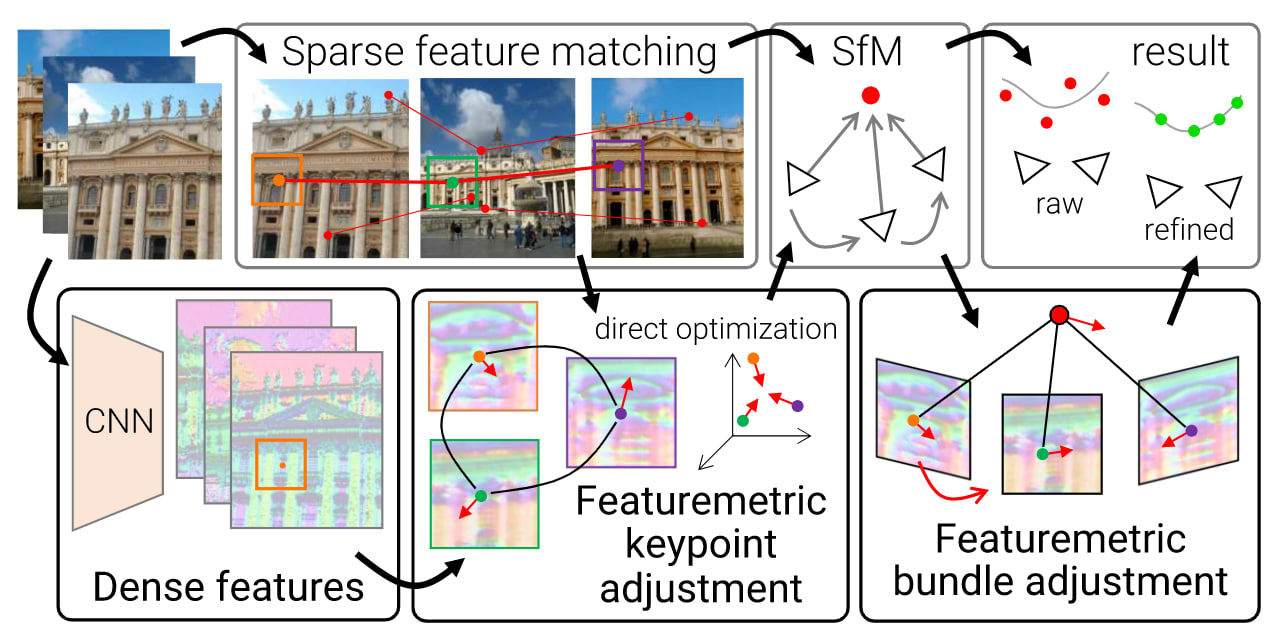
\includegraphics[width=\textwidth,height=\textheight,keepaspectratio]{images/pixel_perfect.jpg}
    \caption{Paper: Pixel-Perfect Structure-from-Motion with Featuremetric Refinement, \cite{lindenberger2021pixsfm}}
    \end{figure}

    They use the initial idea of \cite{Dusmanu2020Multi} that separates the tracks for each keypoint, and
    adjusts their locations by optimizing the geometric cost over the input images in which the keypoint
    is seen. \cite{Dusmanu2020Multi} improved SfM, but has limited accuracy and scalability. To solve that, This paper proposes
    a feature map for each image using convolution neural networks. The feature map condenses the dense
    information from surrounding pixels into a vector for each pixel. The reason behind this step is the
    fact that refining the position of the keypoint is a local operation, not based solely on the pixel value, and the
    dense information only needs to be locally accurate and invariant but not globally discriminative.
    For the first stage, i.e. keypoint adjustment refinement, the locations of 2D keypoints belonging to the same
    track j is refined by optimizing its featuremetric consistency along tentative matches.

    The error between image intensities at two sparse observations is $r &= I_{i}[p_{u}]-I_{j}[p_{v}]$. $I_{i}$ refers
    to the images i-th, and $p_{u}$ refers to u-th pixel's intensity.
    The flow between two points in an image can be inferred from the local image derivatives through a gradient descent update:
    \[ T_{v\rightarrow u}[p_{v}] \propto -\frac{\partial I_{j}}{\partial p} [p_{v}]^\top .r \]

    This can be used to optimize the photometric error. However, as it is said above, the feature map values are used
    instead of direct pixel intensities. Therefore, the simplified loss function used to adjust the locations of 2D keypoints
    belonging to the same track j:

    \[ E &= \sum_{(u,v) \in M_{j}}\lVert F_{u}[p_{u}] - F_{v}[p_{v}]\rVert \]

    In comparison to \cite{Dusmanu2020Multi}, optimizing by the cost of feature maps instead of the patch neighboring
    pixels has better efficiency.


    In the second stage, i.e. bundle adjustment refinement, the typical approach uses the euclidean distance between the point and
    its reprojected 3D from another view. However, this paper considers the difference between the feature vectors
    of the point and the feature vector of the point where the 3D point is reprojected. For each track j, the error
    between its observations and a reference appearance $f_{j}$ is as follows:

    \[ E &= \sum_{j} \sum_{(i,u) \in \tau_{j}}\lVert F_{i}[ \prod (R_{i}P_{j} + t_{i},C_{i})] - f^j\rVert_{\gamma} \]


    Also, instead of acquiring the cost equation for each pair of views, one image is considered as a reference,
    and the cost equations are written between the reference image and the rest of the views. it reduces the number
    of residuals from $O(N^2)$ to $O(N)$. This is not good for sequential video frames. Because newer frames will be
    too far from the reference image. However, it is achievable if the new input is a batch of new images, and
    the refinement is applied to each batch separately.


    As it is mentioned earlier, this paper can be integrated with other approaches. In their experiment,
    \cite{revaud2019r2d2}, \cite{detone2018superpoint}, \cite{dusmanu2019d2net}, and \cite{detone2018superpoint}
    are used as base feature detectors, and then applied refinement. In ETH3D dataset, \cite{Schops_2019_CVPR},
    it is reported that accuracy is improved with an average of 10 to 15 percent for each base feature detector.
    And, the runtime is decreased significantly in comparison to \cite{Dusmanu2020Multi}.

    In order to verify that this paper can actually refine the reconstruction, a test dataset is
    created from a cereal box on a table, and dense 3D point cloud (\ref{fig:cereal}) is obtained by COLMAP (left screenshots)
    and refined by pixel perfect (right screenshots). It can be clearly seen that their approach is promising"

    \begin{figure}
    \centering
    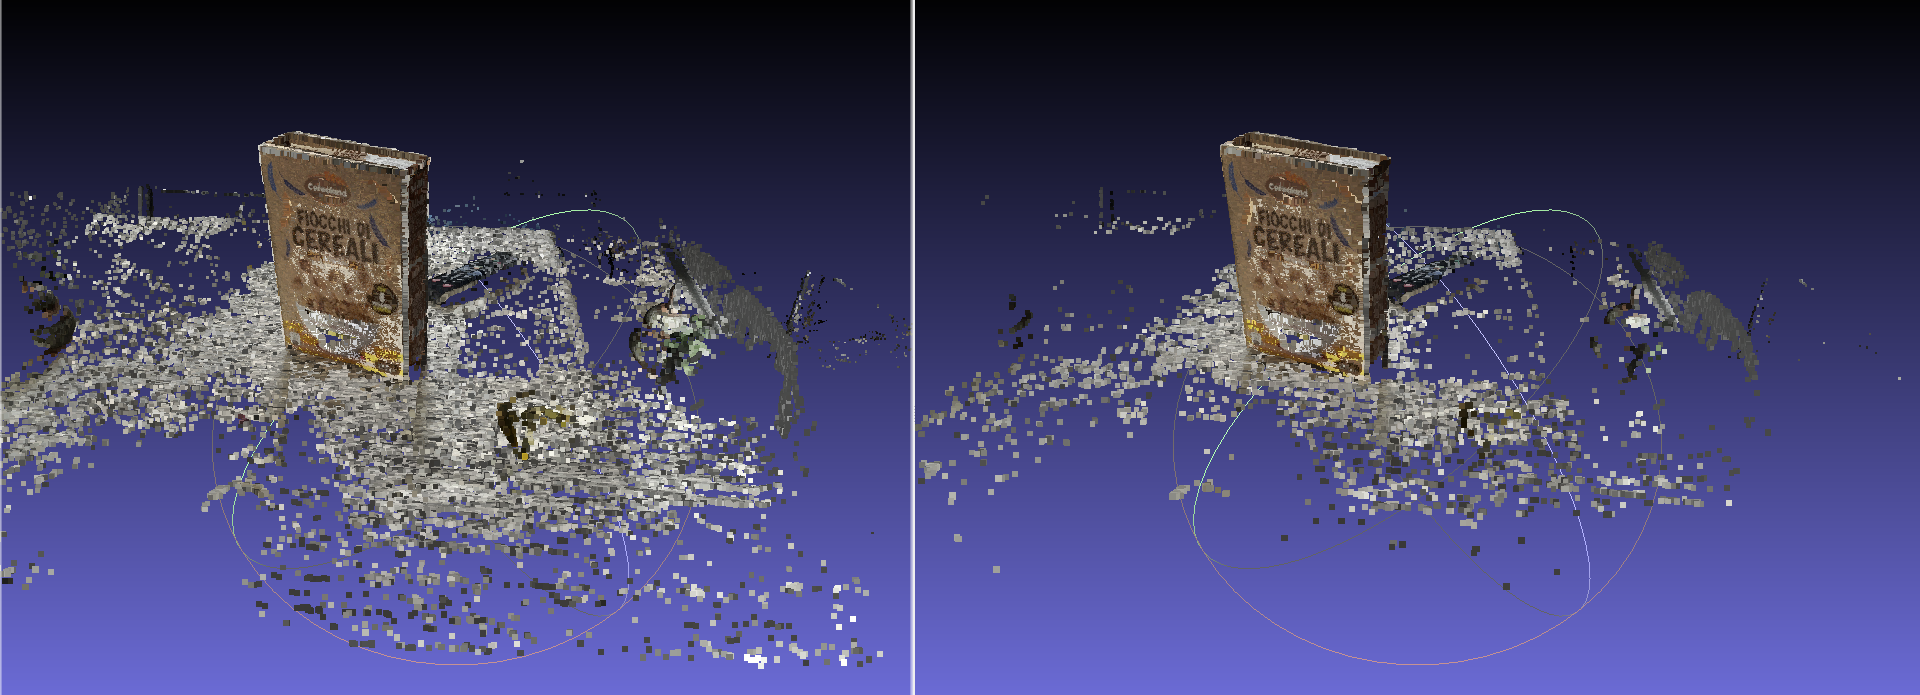
\includegraphics[width=\textwidth,height=\textheight,keepaspectratio]{images/cereal.1.png}
    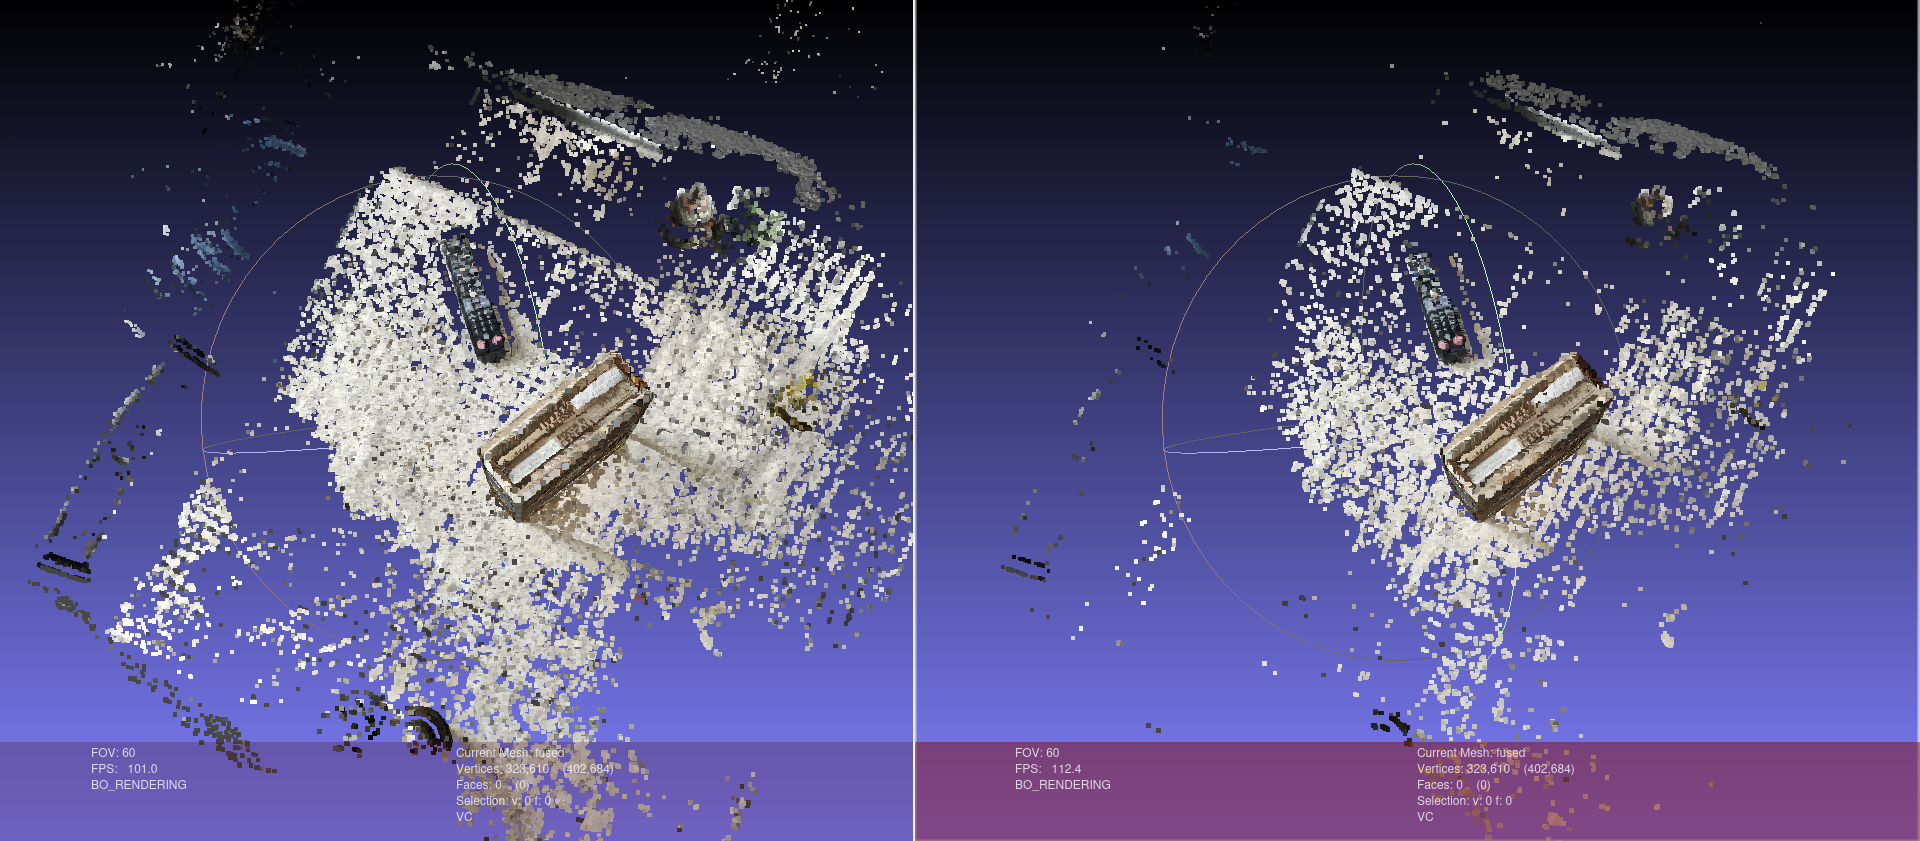
\includegraphics[width=\textwidth,height=\textheight,keepaspectratio]{images/cereal.2.png}
    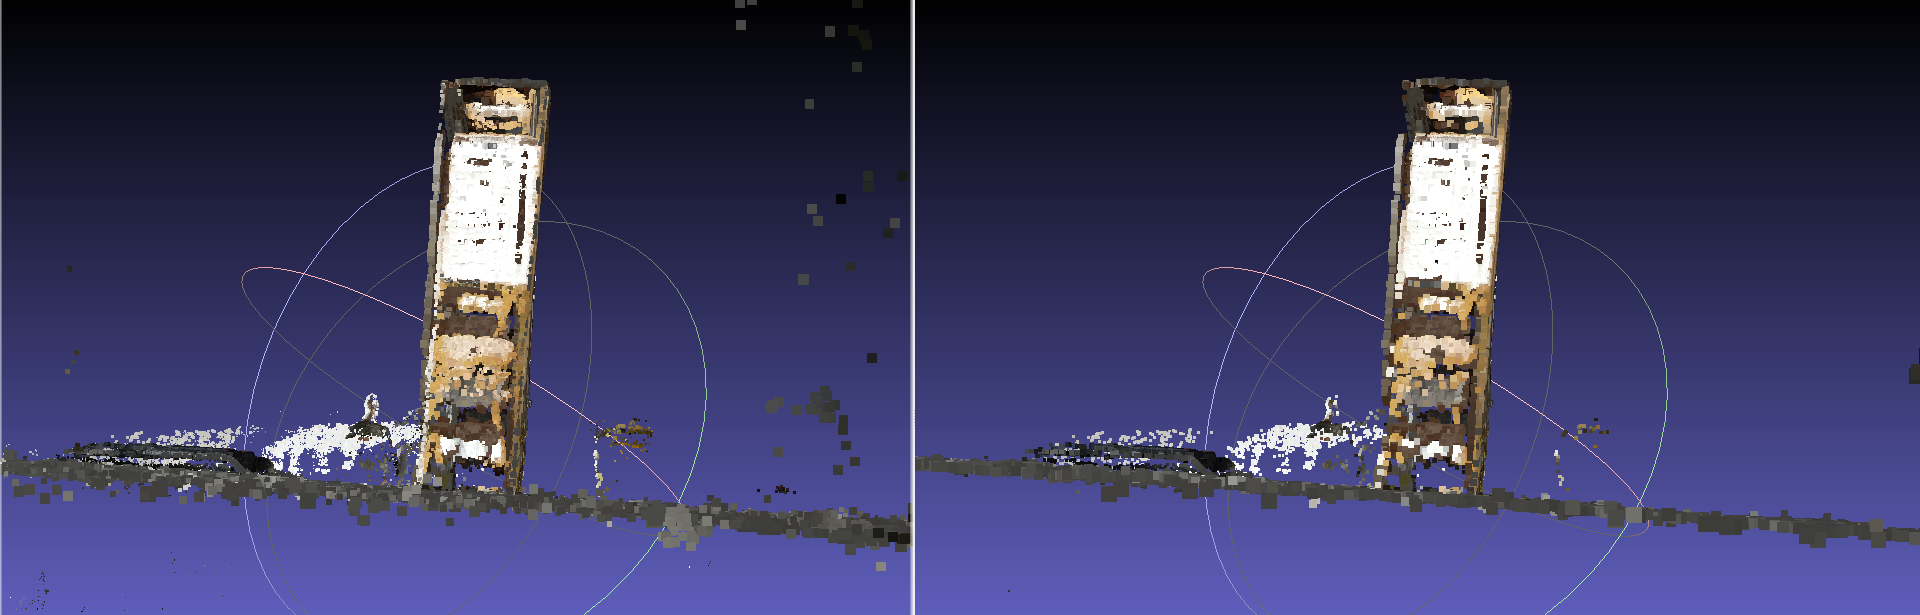
\includegraphics[width=\textwidth,height=\textheight,keepaspectratio]{images/cereal.3.png}
    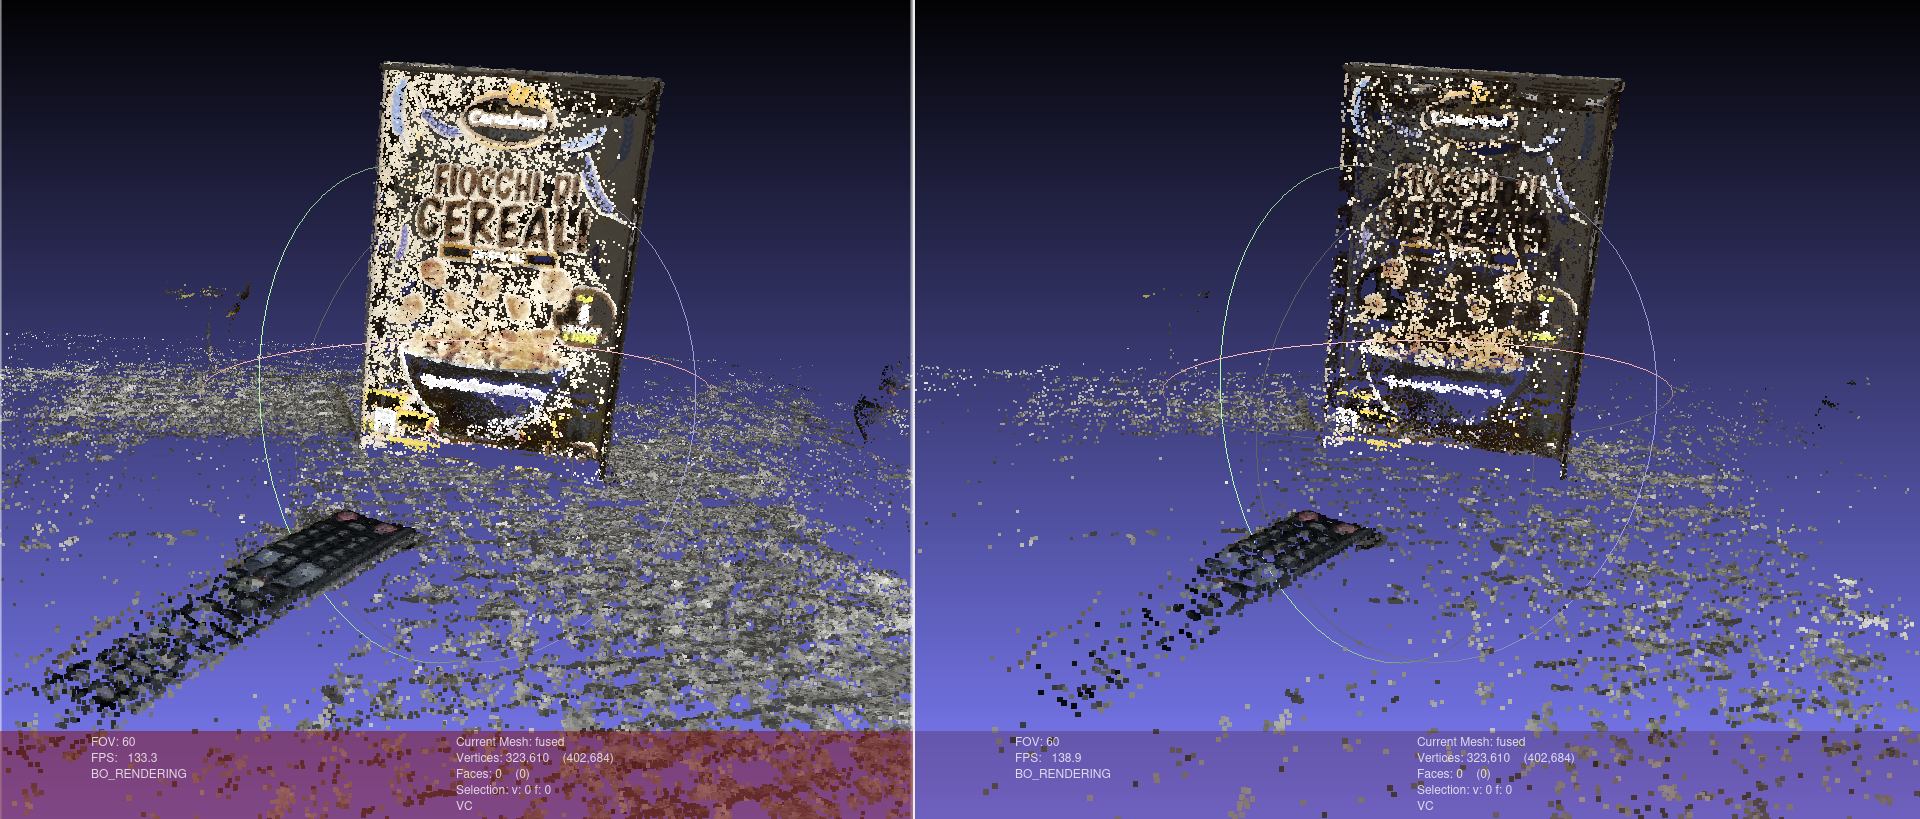
\includegraphics[width=\textwidth,height=\textheight,keepaspectratio]{images/cereal.4.png}
    \caption{Compare The point clouds before and after refinement}
    \label{fig:cereal}
    \end{figure}


\end{document}
